%% Manuscript for Applied Energy (Elsevier CAS double-column template, cas-dc).
%% Every number in this file is a macro from numbers.tex and every data table is a file in tables/,
%% both generated by scripts/make_numbers.py from the repository results (results/paper).
%% Re-run the script after any change of the results, then compile:  latexmk -pdf manuscript

\documentclass[a4paper,fleqn]{cas-dc}

\usepackage[numbers,sort&compress]{natbib}
\usepackage{amsmath,amssymb}
\usepackage{graphicx}
\usepackage{xspace}
\usepackage{eurosym}
\usepackage{tikz}
\usepackage{xurl}
\usetikzlibrary{arrows.meta,positioning,fit,backgrounds}
\hypersetup{hidelinks}

% generated by scripts/make_numbers.py - do not edit
\newcommand{\Ecap}{72\xspace}
\newcommand{\Ebase}{288\xspace}
\newcommand{\socmin}{10\xspace}
\newcommand{\socmax}{90\xspace}
\newcommand{\etabatt}{0.95\xspace}
\newcommand{\pchmax}{24\xspace}
\newcommand{\pdismax}{24\xspace}
\newcommand{\cdegEurMWh}{20\xspace}
\newcommand{\cdegBaseEurMWh}{68.7\xspace}
\newcommand{\pvrated}{30\xspace}
\newcommand{\pveff}{0.92\xspace}
\newcommand{\windarea}{0.32\xspace}
\newcommand{\windcp}{0.20\xspace}
\newcommand{\windcutin}{1\xspace}
\newcommand{\windrated}{8\xspace}
\newcommand{\windcutout}{12\xspace}
\newcommand{\windratedpower}{20.1\xspace}
\newcommand{\sigmaref}{50.1\xspace}
\newcommand{\horizon}{96\xspace}
\newcommand{\dtmin}{15\xspace}
\newcommand{\replansteps}{4\xspace}
\newcommand{\replanmin}{60\xspace}
\newcommand{\unitpower}{24\xspace}
\newcommand{\unittime}{30\xspace}
\newcommand{\fixedcountw}{16.8\xspace}
\newcommand{\violPenalty}{0.05\xspace}
\newcommand{\solverftol}{10^{-7}\xspace}
\newcommand{\lat}{48.088\xspace}
\newcommand{\lon}{19.910\xspace}
\newcommand{\tilt}{35\xspace}
\newcommand{\startCal}{2026-06-16\xspace}
\newcommand{\stopCal}{2026-07-06\xspace}
\newcommand{\daysCal}{21\xspace}
\newcommand{\startTun}{2026-07-07\xspace}
\newcommand{\stopTun}{2026-08-10\xspace}
\newcommand{\daysTun}{35\xspace}
\newcommand{\startDev}{2026-08-11\xspace}
\newcommand{\stopDev}{2026-09-01\xspace}
\newcommand{\daysDev}{22\xspace}
\newcommand{\startFin}{2026-09-02\xspace}
\newcommand{\stopFin}{2026-10-15\xspace}
\newcommand{\daysFin}{44\xspace}
\newcommand{\rmseCal}{1.57\xspace}
\newcommand{\priceCal}{142\xspace}
\newcommand{\renCal}{3.99\xspace}
\newcommand{\demCal}{4.90\xspace}
\newcommand{\rmseTun}{1.59\xspace}
\newcommand{\priceTun}{130\xspace}
\newcommand{\renTun}{6.07\xspace}
\newcommand{\demTun}{8.16\xspace}
\newcommand{\rmseDev}{1.29\xspace}
\newcommand{\priceDev}{154\xspace}
\newcommand{\renDev}{3.18\xspace}
\newcommand{\demDev}{5.22\xspace}
\newcommand{\rmseFin}{1.19\xspace}
\newcommand{\priceFin}{190\xspace}
\newcommand{\renFin}{2.83\xspace}
\newcommand{\demFin}{10.44\xspace}
\newcommand{\weatherStart}{2025-06-01\xspace}
\newcommand{\heldout}{2026-06-16\xspace}
\newcommand{\gprsamples}{5000\xspace}
\newcommand{\calhours}{504\xspace}
\newcommand{\calrmse}{1.67\xspace}
\newcommand{\calrmssigma}{1.24\xspace}
\newcommand{\covRawOne}{66.5\xspace}
\newcommand{\covRawTwo}{88.9\xspace}
\newcommand{\sigmascale}{1.345\xspace}
\newcommand{\phihour}{0.54\xspace}
\newcommand{\phistep}{0.857\xspace}
\newcommand{\swcorr}{-0.047\xspace}
\newcommand{\covDevCAllOne}{80.1\xspace}
\newcommand{\covDevCAllTwo}{96.6\xspace}
\newcommand{\rtsDevCAll}{1.04\xspace}
\newcommand{\covDevCHardOne}{64.6\xspace}
\newcommand{\covDevCHardTwo}{91.7\xspace}
\newcommand{\rtsDevCHard}{1.36\xspace}
\newcommand{\covDevCOtherOne}{85.9\xspace}
\newcommand{\covDevCOtherTwo}{98.4\xspace}
\newcommand{\rtsDevCOther}{0.82\xspace}
\newcommand{\covDevWAllOne}{77.3\xspace}
\newcommand{\covDevWAllTwo}{96.4\xspace}
\newcommand{\rtsDevWAll}{0.62\xspace}
\newcommand{\covDevWHardOne}{63.2\xspace}
\newcommand{\covDevWHardTwo}{92.4\xspace}
\newcommand{\rtsDevWHard}{1.16\xspace}
\newcommand{\covDevWOtherOne}{82.6\xspace}
\newcommand{\covDevWOtherTwo}{97.9\xspace}
\newcommand{\rtsDevWOther}{0.43\xspace}
\newcommand{\covFinCAllOne}{82.5\xspace}
\newcommand{\covFinCAllTwo}{96.3\xspace}
\newcommand{\rtsFinCAll}{0.94\xspace}
\newcommand{\covFinCHardOne}{69.3\xspace}
\newcommand{\covFinCHardTwo}{90.2\xspace}
\newcommand{\rtsFinCHard}{1.27\xspace}
\newcommand{\covFinCOtherOne}{86.9\xspace}
\newcommand{\covFinCOtherTwo}{98.4\xspace}
\newcommand{\rtsFinCOther}{0.75\xspace}
\newcommand{\covFinWAllOne}{74.0\xspace}
\newcommand{\covFinWAllTwo}{92.8\xspace}
\newcommand{\rtsFinWAll}{1.11\xspace}
\newcommand{\covFinWHardOne}{59.8\xspace}
\newcommand{\covFinWHardTwo}{83.7\xspace}
\newcommand{\rtsFinWHard}{1.33\xspace}
\newcommand{\covFinWOtherOne}{78.8\xspace}
\newcommand{\covFinWOtherTwo}{95.8\xspace}
\newcommand{\rtsFinWOther}{0.95\xspace}
\newcommand{\trials}{30\xspace}
\newcommand{\initpoints}{8\xspace}
\newcommand{\frontDet}{5\xspace}
\newcommand{\frontDetbo}{4\xspace}
\newcommand{\frontUa}{7\xspace}
\newcommand{\episodes}{4\xspace}
\newcommand{\episodeDays}{2\xspace}
\newcommand{\episodeList}{07--08 Jul, 18--19 Jul, 29--30 Jul, 09--10 Aug\xspace}
\newcommand{\thrPrimary}{0.5\xspace}
\newcommand{\thrSecondary}{1.0\xspace}
\newcommand{\prereqDate}{2026-10-23\xspace}
\newcommand{\selDet}{t05\xspace}
\newcommand{\selDevDetCost}{0.5113\xspace}
\newcommand{\selDevDetViol}{7.02\xspace}
\newcommand{\selBo}{t13\xspace}
\newcommand{\selDevBoCost}{0.5125\xspace}
\newcommand{\selDevBoViol}{0.45\xspace}
\newcommand{\selUa}{t17\xspace}
\newcommand{\selDevUaCost}{0.5124\xspace}
\newcommand{\selDevUaViol}{0.11\xspace}
\newcommand{\selUaSec}{t24\xspace}
\newcommand{\devFrontPoints}{5\xspace}
\newcommand{\devFrontUa}{4\xspace}
\newcommand{\devPoints}{16\xspace}
\newcommand{\uaFifteenTun}{0.0016\xspace}
\newcommand{\uaFifteenDev}{28.8\xspace}
\newcommand{\rankCorr}{0.24\xspace}
\newcommand{\wDetx}{7.04\times10^{-5}\xspace}
\newcommand{\wDetff}{8.90\times10^{-3}\xspace}
\newcommand{\wDetdu}{4\times10^{-9}\xspace}
\newcommand{\wBox}{1.91\times10^{-5}\xspace}
\newcommand{\wBoff}{8.05\times10^{-2}\xspace}
\newcommand{\wBodu}{1\times10^{-9}\xspace}
\newcommand{\backoff}{0.019\xspace}
\newcommand{\backoffPct}{1.9\xspace}
\newcommand{\wUax}{3.64\times10^{-5}\xspace}
\newcommand{\wUaff}{1.09\times10^{-2}\xspace}
\newcommand{\wUadu}{1\times10^{-9}\xspace}
\newcommand{\lambdaUa}{2.55\xspace}
\newcommand{\zUa}{1.53\xspace}
\newcommand{\alphaUa}{6.3\xspace}
\newcommand{\finDaysBoot}{44\xspace}
\newcommand{\finGridCost}{2.0195\xspace}
\newcommand{\finGridViol}{0.00\xspace}
\newcommand{\finGridMaxViol}{0.00\xspace}
\newcommand{\finGridBmsCost}{2.0195\xspace}
\newcommand{\finGridProt}{0\xspace}
\newcommand{\finGridExtra}{0.00\xspace}
\newcommand{\finGridCyc}{0.00\xspace}
\newcommand{\finRuleCost}{1.7430\xspace}
\newcommand{\finRuleViol}{0.00\xspace}
\newcommand{\finRuleMaxViol}{0.00\xspace}
\newcommand{\finRuleBmsCost}{1.7430\xspace}
\newcommand{\finRuleProt}{0\xspace}
\newcommand{\finRuleExtra}{0.00\xspace}
\newcommand{\finRuleCyc}{0.72\xspace}
\newcommand{\finDetCost}{1.5152\xspace}
\newcommand{\finDetViol}{10.74\xspace}
\newcommand{\finDetMaxViol}{1.26\xspace}
\newcommand{\finDetBmsCost}{1.5192\xspace}
\newcommand{\finDetProt}{108\xspace}
\newcommand{\finDetExtra}{7.58\xspace}
\newcommand{\finDetCyc}{0.67\xspace}
\newcommand{\finDetSolver}{94.0\xspace}
\newcommand{\finDetSolve}{1.13\xspace}
\newcommand{\finBoCost}{1.5171\xspace}
\newcommand{\finBoViol}{0.15\xspace}
\newcommand{\finBoMaxViol}{0.01\xspace}
\newcommand{\finBoBmsCost}{1.5198\xspace}
\newcommand{\finBoProt}{42\xspace}
\newcommand{\finBoExtra}{0.93\xspace}
\newcommand{\finBoCyc}{0.67\xspace}
\newcommand{\finBoSolver}{92.3\xspace}
\newcommand{\finBoSolve}{1.10\xspace}
\newcommand{\finUaCost}{1.5169\xspace}
\newcommand{\finUaViol}{0.20\xspace}
\newcommand{\finUaMaxViol}{0.09\xspace}
\newcommand{\finUaBmsCost}{1.5200\xspace}
\newcommand{\finUaProt}{49\xspace}
\newcommand{\finUaExtra}{2.62\xspace}
\newcommand{\finUaCyc}{0.67\xspace}
\newcommand{\finUaSolver}{91.2\xspace}
\newcommand{\finUaSolve}{0.52\xspace}
\newcommand{\finRhoCost}{1.5143\xspace}
\newcommand{\finRhoViol}{12.91\xspace}
\newcommand{\finRhoMaxViol}{1.40\xspace}
\newcommand{\finRhoBmsCost}{1.5184\xspace}
\newcommand{\finRhoProt}{126\xspace}
\newcommand{\finRhoExtra}{8.34\xspace}
\newcommand{\finRhoCyc}{0.67\xspace}
\newcommand{\finRhoSolver}{93.6\xspace}
\newcommand{\finRhoSolve}{1.11\xspace}
\newcommand{\finMarginCost}{1.5169\xspace}
\newcommand{\finMarginViol}{0.35\xspace}
\newcommand{\finMarginMaxViol}{0.06\xspace}
\newcommand{\finMarginBmsCost}{1.5200\xspace}
\newcommand{\finMarginProt}{50\xspace}
\newcommand{\finMarginExtra}{2.52\xspace}
\newcommand{\finMarginCyc}{0.67\xspace}
\newcommand{\finMarginSolver}{91.2\xspace}
\newcommand{\finMarginSolve}{0.52\xspace}
\newcommand{\finSecCost}{1.5155\xspace}
\newcommand{\finSecViol}{3.88\xspace}
\newcommand{\finSecMaxViol}{0.91\xspace}
\newcommand{\finSecBmsCost}{1.5186\xspace}
\newcommand{\finSecProt}{65\xspace}
\newcommand{\finSecExtra}{3.30\xspace}
\newcommand{\finSecCyc}{0.67\xspace}
\newcommand{\finSecSolver}{91.8\xspace}
\newcommand{\finSecSolve}{0.50\xspace}
\newcommand{\finOracleCost}{1.4829\xspace}
\newcommand{\finOracleViol}{0.06\xspace}
\newcommand{\finOracleMaxViol}{0.00\xspace}
\newcommand{\finOracleBmsCost}{1.4904\xspace}
\newcommand{\finOracleProt}{101\xspace}
\newcommand{\finOracleExtra}{5.31\xspace}
\newcommand{\finOracleCyc}{0.72\xspace}
\newcommand{\finOracleSolver}{97.0\xspace}
\newcommand{\finOracleSolve}{0.26\xspace}
\newcommand{\finGridSaveUa}{24.9\xspace}
\newcommand{\finRuleSaveUa}{13.0\xspace}
\newcommand{\finOracleGap}{2.2\xspace}
\newcommand{\finDetOracleGap}{2.2\xspace}
\newcommand{\finDemand}{10.44\xspace}
\newcommand{\finRenew}{2.83\xspace}
\newcommand{\btDetViolPct}{98\xspace}
\newcommand{\btDetViolP}{1.000\xspace}
\newcommand{\btDetCostPct}{0.09\xspace}
\newcommand{\btDetCostP}{0.294\xspace}
\newcommand{\btDetProtPct}{55\xspace}
\newcommand{\btDetProtP}{1.000\xspace}
\newcommand{\btDetExtraPct}{65\xspace}
\newcommand{\btDetExtraP}{1.000\xspace}
\newcommand{\btDetBmsCostPct}{0.03\xspace}
\newcommand{\btDetBmsCostP}{0.435\xspace}
\newcommand{\btBoViolPct}{35\xspace}
\newcommand{\btBoViolP}{0.057\xspace}
\newcommand{\btBoCostPct}{0.00\xspace}
\newcommand{\btBoCostP}{0.514\xspace}
\newcommand{\btBoProtPct}{17\xspace}
\newcommand{\btBoProtP}{0.116\xspace}
\newcommand{\btBoExtraPct}{181\xspace}
\newcommand{\btBoExtraP}{0.000\xspace}
\newcommand{\btBoBmsCostPct}{0.02\xspace}
\newcommand{\btBoBmsCostP}{0.436\xspace}
\newcommand{\btRhoViolPct}{98\xspace}
\newcommand{\btRhoViolP}{1.000\xspace}
\newcommand{\btRhoCostPct}{0.17\xspace}
\newcommand{\btRhoCostP}{0.001\xspace}
\newcommand{\btRhoProtPct}{61\xspace}
\newcommand{\btRhoProtP}{1.000\xspace}
\newcommand{\btRhoExtraPct}{69\xspace}
\newcommand{\btRhoExtraP}{1.000\xspace}
\newcommand{\btRhoBmsCostPct}{0.11\xspace}
\newcommand{\btRhoBmsCostP}{0.006\xspace}
\newcommand{\btMarginViolPct}{42\xspace}
\newcommand{\btMarginViolP}{0.900\xspace}
\newcommand{\btMarginCostPct}{0.00\xspace}
\newcommand{\btMarginCostP}{0.644\xspace}
\newcommand{\btMarginProtPct}{2.00\xspace}
\newcommand{\btMarginProtP}{0.655\xspace}
\newcommand{\btMarginExtraPct}{3.73\xspace}
\newcommand{\btMarginExtraP}{0.194\xspace}
\newcommand{\btMarginBmsCostPct}{0.00\xspace}
\newcommand{\btMarginBmsCostP}{0.460\xspace}
\newcommand{\btOracleViolPct}{252\xspace}
\newcommand{\btOracleViolP}{0.166\xspace}
\newcommand{\btOracleCostPct}{2.21\xspace}
\newcommand{\btOracleCostP}{0.000\xspace}
\newcommand{\btOracleProtPct}{51\xspace}
\newcommand{\btOracleProtP}{1.000\xspace}
\newcommand{\btOracleExtraPct}{51\xspace}
\newcommand{\btOracleExtraP}{0.999\xspace}
\newcommand{\btOracleBmsCostPct}{1.91\xspace}
\newcommand{\btOracleBmsCostP}{0.000\xspace}
\newcommand{\devAblDetViol}{14.10\xspace}
\newcommand{\devAblDetProt}{272\xspace}
\newcommand{\devAblBoViol}{0.45\xspace}
\newcommand{\devAblBoProt}{138\xspace}
\newcommand{\devAblUaViol}{4.38\xspace}
\newcommand{\devAblUaProt}{163\xspace}
\newcommand{\devAblRhoViol}{7.77\xspace}
\newcommand{\devAblRhoProt}{180\xspace}
\newcommand{\devAblMarginViol}{5.27\xspace}
\newcommand{\devAblMarginProt}{163\xspace}
\newcommand{\devAblOracleViol}{0.09\xspace}
\newcommand{\devAblOracleProt}{263\xspace}
\newcommand{\solverFailMin}{5.5\xspace}
\newcommand{\solverFailMax}{7.4\xspace}
\newcommand{\onsetsTotal}{95\xspace}
\newcommand{\onsetsFailed}{0\xspace}
\newcommand{\violFailedMin}{15\xspace}
\newcommand{\violFailedMax}{72\xspace}
\newcommand{\iterFailedMin}{34\xspace}
\newcommand{\iterFailedMax}{74\xspace}
\newcommand{\iterOkMin}{7\xspace}
\newcommand{\iterOkMax}{14\xspace}
\newcommand{\recDetBefore}{7.02\xspace}
\newcommand{\recDetAfter}{6.10\xspace}
\newcommand{\recDetSolBefore}{94.5\xspace}
\newcommand{\recDetSolAfter}{100.0\xspace}
\newcommand{\recDetCostChange}{0.00\xspace}
\newcommand{\recBoBefore}{0.45\xspace}
\newcommand{\recBoAfter}{0.15\xspace}
\newcommand{\recBoSolBefore}{92.6\xspace}
\newcommand{\recBoSolAfter}{100.0\xspace}
\newcommand{\recBoCostChange}{0.01\xspace}
\newcommand{\recUaBefore}{0.11\xspace}
\newcommand{\recUaAfter}{0.11\xspace}
\newcommand{\recUaSolBefore}{93.4\xspace}
\newcommand{\recUaSolAfter}{98.1\xspace}
\newcommand{\recUaCostChange}{0.00\xspace}
\newcommand{\kappaSigma}{0.31\xspace}
\newcommand{\mapLowMaxViol}{0.64\xspace}
\newcommand{\mapLowCostAbs}{1.0\xspace}
\newcommand{\mapHighBoMin}{2.8\xspace}
\newcommand{\mapHighBoMax}{19.1\xspace}
\newcommand{\mapHighUaMin}{0.04\xspace}
\newcommand{\mapHighUaMax}{1.25\xspace}
\newcommand{\mapHighRatioMin}{6\xspace}
\newcommand{\mapHighRatioMax}{77\xspace}
\newcommand{\mapHighCostMin}{0.1\xspace}
\newcommand{\mapHighCostMax}{0.6\xspace}
\newcommand{\mapLowThr}{0.023\xspace}
\newcommand{\mapHighThr}{0.047\xspace}
\newcommand{\mapCells}{10\xspace}
\newcommand{\rEbase}{0.023\xspace}
\newcommand{\oldOutBo}{143.3\xspace}
\newcommand{\mapBaseBoSingle}{0.18\xspace}
\newcommand{\newOutBo}{0.64\xspace}
\newcommand{\oldOutUa}{58.7\xspace}
\newcommand{\newOutUa}{0.23\xspace}
\newcommand{\chanceFacMin}{36\xspace}
\newcommand{\chanceFacMax}{106\xspace}
\newcommand{\sigRatioMed}{2.7\xspace}
\newcommand{\sigRatioNinetyFive}{4.2\xspace}
\newcommand{\rhoMinUa}{0.983\xspace}
\newcommand{\rhoMinDefault}{0.13\xspace}
\newcommand{\frontLowLambda}{5\xspace}
\newcommand{\frontLambdaMax}{2{,}811\xspace}
\newcommand{\hardDay}{18 August 2026\xspace}
\newcommand{\hardErrWh}{38.0\xspace}
\newcommand{\hardDetMinSoc}{7.6\xspace}
\newcommand{\hardBoMinSoc}{9.5\xspace}
\newcommand{\hardUaMinSoc}{9.7\xspace}
\newcommand{\violNoise}{0.01\xspace}
\newcommand{\kappaAmplified}{0.61\xspace}
\newcommand{\varCells}{4\xspace}
\newcommand{\varConstRatioMin}{2.3\xspace}
\newcommand{\varConstRatioMax}{3.8\xspace}
\newcommand{\varAmpLower}{3\xspace}
\newcommand{\varAmpRatioMin}{3.3\xspace}
\newcommand{\varAmpRatioMax}{5.3\xspace}
\newcommand{\varAmpWorseUa}{0.036\xspace}
\newcommand{\varAmpWorseAmp}{0.089\xspace}
\newcommand{\varCostSpreadMax}{0.11\xspace}
\newcommand{\varBaseConst}{0.34\xspace}
\newcommand{\varBaseUa}{0.11\xspace}
\newcommand{\varBaseAmp}{0.024\xspace}
\newcommand{\varConstBelowBo}{3\xspace}
\newcommand{\gridOnlyDev}{0.8294\xspace}
\newcommand{\capSSave}{0.259\xspace}
\newcommand{\capSPerWh}{7.2\xspace}
\newcommand{\capSShare}{71\xspace}
\newcommand{\capMSave}{0.317\xspace}
\newcommand{\capMPerWh}{4.4\xspace}
\newcommand{\capMShare}{87\xspace}
\newcommand{\capLSave}{0.364\xspace}
\newcommand{\capLPerWh}{2.5\xspace}
\newcommand{\capLShare}{100\xspace}
\newcommand{\capMargMS}{1.6\xspace}
\newcommand{\capMargLM}{0.65\xspace}
\newcommand{\capShareMin}{69\xspace}
\newcommand{\capShareMax}{72\xspace}

\makeatletter\newcommand\inputtab[1]{\@@input #1 }\makeatother

\newcommand{\pph}{\,pp$\cdot$h\xspace}
\xspaceaddexceptions{\, \pph \% ] \texttimes}
\newcommand{\DET}{DET\xspace}
\newcommand{\DETBO}{DET-BO\xspace}
\newcommand{\UA}{UA-MPC\xspace}
\newcommand{\rE}{r_{\mathrm{E}}}
\newcommand{\rP}{r_{\mathrm{P}}}

\begin{document}
\let\WriteBookmarks\relax
\def\floatpagepagefraction{1}
\def\textpagefraction{.001}

\shorttitle{Uncertainty-aware MPC as a self-adjusting safety margin}
\shortauthors{J. Szeles and L. Deszát}

\title[mode = title]{Uncertainty-aware MPC as a self-adjusting safety margin for renewable-powered production cells}

\author[1]{József Szeles}
\cormark[1]
\ead{} % TODO: corresponding e-mail address
\credit{Conceptualization, Methodology, Software, Validation, Formal analysis, Investigation, Data curation, Writing -- original draft, Visualization}

\author[1]{Laura Deszát}
\credit{Conceptualization, Methodology, Software, Investigation, Writing -- review \& editing}

% TODO: complete the address (street, city, postcode) of the department
\affiliation[1]{organization={Department of System Engineering, University of Pannonia},
            country={Hungary}}

\cortext[1]{Corresponding author}

\begin{abstract}
Battery schedules computed by model predictive control (MPC) from renewable forecasts violate their state-of-charge (SoC) limits when the forecast is wrong. The usual remedies, a stochastic MPC that tightens the limits by the forecast uncertainty and a simple constant SoC back-off, are rarely compared. We study a renewable-powered production cell (\pvrated\,W PV, \windratedpower\,W wind, \Ecap\,Wh battery, production-schedule load) whose forecast comes from a physical model corrected by Gaussian-process regression. The forecast standard deviation is calibrated on held-out days and enters the MPC twice: as a confidence weight on the forecast-tracking term of the cost and as a chance-constrained SoC margin accumulated over the AR(1)-correlated forecast errors until the next re-planning. Deterministic MPC, deterministic MPC with a constant back-off and the uncertainty-aware MPC received the same multi-objective Bayesian tuning budget; their operating points were selected by a rule fixed in advance and evaluated once on a \daysFin-day final test in closed-loop replay. The uncertainty-aware MPC cut SoC-band violations by \btDetViolPct\,\% and battery-protection interventions by \btDetProtPct\,\% compared with deterministic MPC, at equal cost. It did not differ significantly from the constant back-off in the setting that back-off was tuned for. When battery capacity, forecast-error level or re-planning interval changed, the same weights kept the band (\mapHighUaMin--\mapHighUaMax\pph over \daysDev days) while the constant back-off did not (\mapHighBoMin--\mapHighBoMax\pph), at \mapHighCostMin--\mapHighCostMax\,\% extra cost. A simple ratio, the 95\,\% energy deficit until the next re-plan over the usable capacity, indicates in advance when a constant back-off stops being enough. The time variability of the uncertainty carries part of this information: with the same mean standard deviation held constant in time, the violation rose \varConstRatioMin--\varConstRatioMax-fold. Small batteries, which earn the most per watt-hour (a \capSShare\,\% share of the saving of a four times larger battery), are where the self-adjusting margin is needed most.
\end{abstract}

\begin{graphicalabstract}
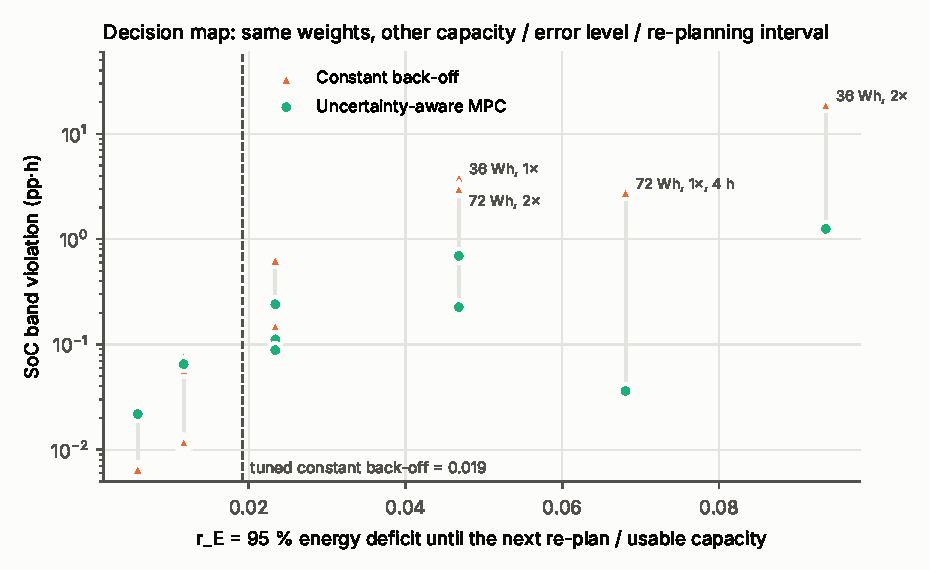
\includegraphics[width=\linewidth]{figures/fig3_decision_map.pdf}
\end{graphicalabstract}

\begin{highlights}
\item Forecast uncertainty enters the MPC cost as confidence weights and a SoC margin
\item Pre-registered final test: \btDetViolPct\,\% fewer SoC violations than deterministic MPC
\item A constant back-off tuned for the setting is as good, but only in that setting
\item An energy-deficit ratio shows when a constant back-off stops being enough
\item Time-varying forecast uncertainty, not only its level, sets the needed margin
\end{highlights}

\begin{keywords}
model predictive control \sep forecast uncertainty \sep chance constraint \sep Gaussian process regression \sep battery storage \sep industrial production \sep constant back-off
\end{keywords}

\maketitle

%% =====================================================================================
\section{Introduction}\label{sec:intro}

Small industrial consumers increasingly combine on-site photovoltaics, small wind turbines and a battery. The battery lets them shift renewable energy to the hours of production and buy grid energy when it is cheap; energy-aware production and industrial demand response pursue the same goal from the load side \cite{gahm2016energy,shoreh2016survey,zhang2016enterprise,golmohamadi2022demand,beier2017energy}. Model predictive control (MPC) is the standard tool for this kind of operation: it plans the battery over a receding horizon from forecasts of the renewable power, the load and the price, applies the first part of the plan and re-plans from the measured state \cite{mayne2000constrained,rawlings2017model,parisio2014mpc,hu2021mpcmicrogrid}.

The plan is only as good as the forecast. When the renewable power falls short of the forecast, the battery delivers energy that the plan had not reserved, and the state of charge (SoC) leaves the band the operator wants to keep it in. In the field this is not a modelling inconvenience: the battery management system (BMS) cuts the discharge at its lower limit, the load falls back on the grid at the current price, and the cell ages faster near its limits. Two remedies are common. Stochastic MPC formulates the SoC limits as chance constraints and tightens them by a quantile of the forecast-error distribution \cite{mesbah2016stochastic,farina2016stochastic,oldewurtel2012use}. The simpler alternative keeps the deterministic MPC and tightens the limits by a constant back-off. Kumar et al.\ \cite{kumar2019benchmarking} compared both for a stationary battery and found that deterministic MPC violates its constraints and that a constant back-off helps only in an ad hoc way.

Two questions remain open for an operator who must choose. First, is an uncertainty-aware MPC better than a constant back-off that has been tuned with the same effort, or only better than a deterministic MPC without any safety margin? Most evaluations compare against the latter. Second, if the two are equivalent in one setting, when do they differ? A constant back-off is a number tuned for one battery, one forecast quality and one re-planning interval; a margin computed from a calibrated forecast uncertainty adjusts itself when these change. The answers also depend on how the comparison is made: closed-loop operation rather than single plans, the same tuning budget for every controller, an operating point chosen before the test, and a test period that is used only once.

Two further aspects make the question practical. Battery capacity is the dominant investment of such a system, and its value shows diminishing returns: the first watt-hours earn the most \cite{weniger2014sizing,quoilin2016quantifying,mulleriyawage2020optimally}, and even a battery much smaller than the worst case covers most fluctuations because large ones are rare \cite{makibar2017relation}. A small battery, however, has the least room for forecast errors. Second, renewable forecast uncertainty is not constant: calm and turbulent periods alternate \cite{widen2015variability,stein2012variability}. A constant margin must be sized for one of them; a margin that follows the forecast uncertainty can be small in calm periods and large in turbulent ones.

This paper answers these questions for a renewable-powered production cell. We ask:
\begin{enumerate}
\item[RQ1] Does a calibrated uncertainty-aware MPC keep the SoC band better than deterministic MPC, without extra cost?
\item[RQ2] Is it better than a constant back-off tuned for the same setting with the same budget?
\item[RQ3] When does the difference between the two appear, and can an operator tell in advance?
\item[RQ4] Does the time variability of the forecast uncertainty matter, beyond its mean level, and what does the margin mean for small batteries?
\end{enumerate}

The contributions are:
\begin{enumerate}
\item An MPC cost function with uncertainty-aware weights. The calibrated forecast standard deviation $\sigma_k$ enters the cost through a confidence factor $\rho_k=1/(1+\lambda(\sigma_k/\sigma_{\mathrm{ref}})^2)$ on the forecast-tracking term, and the constraints through a chance-constrained SoC margin; $\sigma_{\mathrm{ref}}$ makes $\lambda$ independent of the system size. The margin accumulates AR(1)-correlated forecast errors only until the next re-planning, where the measured SoC resets them.
\item A two-channel (solar, wind) Gaussian-process residual forecast whose standard deviation is calibrated on held-out data, with the calibration reported on independent periods.
\item An evaluation protocol: closed-loop replay, equal-budget multi-objective Bayesian tuning of every controller, a four-period split with a pre-registered point-selection rule and a one-shot final test, a constant back-off baseline, ablations, and a three-level violation metric with a BMS plant.
\item A decision map over battery capacity, forecast-error level and re-planning interval, and a ratio $\rE$ that separates the region where a tuned constant back-off is enough from the region where it fails.
\item A variability experiment that keeps the mean forecast standard deviation and changes only its variation in time, and a capacity analysis that links the margin to the economics of small batteries.
\end{enumerate}

Section~\ref{sec:related} positions the work. Section~\ref{sec:system} describes the cell and the data, Section~\ref{sec:method} the forecast, the controller and the evaluation protocol. Section~\ref{sec:results} reports the results, Section~\ref{sec:discussion} discusses them and their limits, and Section~\ref{sec:conclusion} concludes.

%% =====================================================================================
\section{Related work}\label{sec:related}

\paragraph{Deterministic MPC for microgrids and storage} Economic MPC of a battery-supported microgrid with renewable and price forecasts was set out by Parisio et al.\ \cite{parisio2014mpc}; the receding-horizon principle, its stability theory and its economic variant are summarised in \cite{mayne2000constrained,rawlings2017model,angeli2012average,ellis2014tutorial}. Rolling-horizon energy-management systems have been built for microgrids \cite{palmabehnke2013microgrid,silvente2015rolling,kriett2012residential,bruni2015domestic}, for hybrid storage with hydrogen \cite{garciatorres2016hydrogen}, for off-grid systems with the same PV--wind--battery mix as our cell \cite{torreglosa2015energy}, for buildings with PV and storage \cite{tarragona2020model,cai2019aging} and for a commercial site with a cloud-based controller \cite{goldsworthy2022cloud}. Reviews of MPC for microgrids and buildings \cite{hu2021mpcmicrogrid,garciatorres2021mpcfunctionalities,drgona2020allyouneed,serale2018mpc} show that most implementations use point forecasts and rely on re-planning for robustness. This deterministic MPC is the first baseline of this paper. Our formulation follows the same structure (power balance, SoC dynamics, energy and wear cost) for a single production cell, with continuous variables and quadratic terms.

\paragraph{Stochastic, robust and risk-aware MPC} Chance-constrained programming goes back to Charnes and Cooper \cite{charnes1959chance}. In stochastic MPC an individual chance constraint with Gaussian disturbance reduces to tightening the constraint by a quantile times the predicted standard deviation \cite{mesbah2016stochastic,farina2016stochastic,lorenzen2017constraint,kouvaritakis2016model}; scenario methods replace the distribution by samples \cite{calafiore2006scenario,schildbach2014scenario}. Weather-forecast-driven stochastic MPC was demonstrated for buildings \cite{oldewurtel2012use,oldewurtel2014stochastic,parisio2013scenario,parisio2014implementation}, and stochastic or probabilistic energy management for microgrids \cite{velarde2017comparison,silvente2018rolling,cheng2020probabilistic,wu2021mpcev} and storage \cite{arnold2011mpc,kumar2018stochastic}. Robust MPC bounds the worst case instead \cite{bemporad1999robust,mayne2005robust}, also for microgrids and buildings with renewable uncertainty \cite{zhang2013robust,hu2024improved}; risk measures bound the depth of violations \cite{rockafellar2000optimization,narayan2017risk}. Lei et al.\ \cite{lei2021optimal} bound not only the probability but also the depth of SoC violations; this motivates our depth-times-duration metric. In power systems, chance constraints under renewable uncertainty are standard \cite{bienstock2014chance,roald2018chance}. Hewing et al.\ \cite{hewing2020cautious,hewing2020learning} propagate the predictive variance of a Gaussian process (GP) through the horizon to tighten constraints. Mesbah \cite{mesbah2016stochastic} notes that open-loop prediction of the uncertainty is conservative because future feedback is ignored, and Schildbach et al.\ \cite{schildbach2014scenario} show that closed-loop violation rates are far below the open-loop chance level; our margin therefore accumulates the uncertainty only until the next re-plan, and we measure the closed-loop chance level directly.

\paragraph{Back-off baselines and benchmarking} The simplest tightening is a constant back-off. Kumar et al.\ \cite{kumar2019benchmarking} benchmarked stochastic against deterministic MPC for stationary batteries, including a constant back-off, which they call ad hoc. Back-offs computed from GP uncertainty \cite{bradford2020backoffs} and tightening that adapts to time-varying uncertainty \cite{bujarbaruah2021adaptive} make the margin uncertainty-dependent. De Miguel Rodriguez et al.\ \cite{demiguel2026mapping} mapped battery-scheduling performance across data uncertainty, battery design and planning horizon for a deterministic scheduler. None of these gives a rule for when an uncertainty-dependent margin pays off over a constant one tuned with the same effort.

\paragraph{Probabilistic renewable forecasts and their value} Physical, statistical and hybrid PV forecasting are reviewed in \cite{antonanzas2016review,voyant2017machine}, probabilistic PV forecasting in \cite{vandermeer2018review}, wind forecasting for operation in \cite{pinson2013wind}, and the role of forecasts in decisions in \cite{hong2016probabilistic,sweeney2020future}. GP regression provides a predictive distribution at every point \cite{rasmussen2006gaussian} and has been used for probabilistic solar forecasts \cite{najibi2021enhanced}; heteroscedastic GPs let the variance depend on the input \cite{kersting2007most}. A probabilistic forecast is useful only if it is calibrated \cite{gneiting2007probabilistic,gneiting2007scoring}; we calibrate the GP standard deviation on held-out days and report its coverage on independent periods. Price forecasting is reviewed in \cite{weron2014electricity,lago2021forecasting}. For storage, forecast errors have a measurable economic cost: assuming perfect forecasts overstates the value of PV--battery systems \cite{mirletz2023impacts}, the cost of solar forecast errors is substantial \cite{gandhi2024value}, and the use of forecasts in storage operation and sizing is reviewed in \cite{sharma2021use,seervi2021renewable}. Economic MPC has been evaluated with real forecast errors \cite{manzano2022economic}, and forecast-driven decision support for solar microgrids with storage is recent work in this journal \cite{tariq2026pvforecasting}.

\paragraph{Variability of renewable supply} Renewable output varies on all time scales and across space \cite{widen2015variability,engeland2017spacetime,krakauer2017interannual}. Its short-term variability has been quantified by fleet and plant-level models \cite{hoff2010quantifying,mills2010implications,lave2013wavelet} and summarised by the dimensionless variability index \cite{stein2012variability}; forecasting can reduce the battery needed for ramp-rate control \cite{gonzalezmoreno2022pv}. These works describe the variability of the power. We study the variability of the forecast \emph{uncertainty}, $\kappa_\sigma$, and its effect on a margin.

\paragraph{Ratios and the economics of small batteries} Storage design is commonly reduced to dimensionless ratios: self-consumption and self-sufficiency \cite{luthander2015selfconsumption,quoilin2016quantifying,alnaser2021transition}, capacity normalised by annual load or PV size \cite{weniger2014sizing,mason2016energetic}, energy-to-power ratio and C-rate \cite{hesse2017lithium,dowling2020role}, battery size relative to a ramp-rate limit \cite{makibar2017relation} and inverter- or battery-to-PV ratios \cite{diorio2020model}; design-space maps relate storage cost and duration to its value \cite{sepulveda2021design}. Battery costs fall \cite{schmidt2017future,kittner2017energy,schmidt2019projecting,ziegler2021reexamining}, yet capacity remains the main investment \cite{zakeri2015electrical}, ageing adds to it \cite{xu2018factoring,wu2022optimal}, and sizing studies for residential, commercial and grid-connected systems find diminishing returns of capacity \cite{weniger2014sizing,mulleriyawage2020optimally,linssen2017techno,laksahapsoro2025optimisation,secchi2021multi,yang2018bess,zhang2022gridconnected}; system studies reach similar conclusions for the grid \cite{zerrahn2018economics}. Our ratio $\rE$ belongs to this family, but it is an operational ratio: it relates the forecast error that can accumulate before the controller reacts to the capacity, and so tells whether a given margin is enough.

\paragraph{Tuning and evaluation} MPC weights are expensive black-box parameters: one evaluation is a multi-day closed-loop simulation. Bayesian optimisation \cite{shahriari2016taking}, efficient global optimisation with a GP surrogate \cite{jones1998efficient} and its multi-objective variant ParEGO \cite{knowles2006parego} are standard for such problems; GP-based optimisation has tuned controllers in closed loop \cite{marco2016automatic}, and Sorourifar et al.\ \cite{sorourifar2021data} used constrained Bayesian optimisation to tune MPC under uncertainty. We give every controller the same ParEGO budget, so that differences are not differences of tuning effort, and we evaluate on chronologically separated periods \cite{bergmeir2012use,lago2021forecasting}.

Table~\ref{tab:positioning} summarises the closest works. The individual elements are known; the contribution of this paper is their combination and, above all, the comparison against a tuned constant back-off across operating conditions.

\begin{table*}[t]
\caption{Closest works and this paper.}\label{tab:positioning}
\begin{tabular*}{\tblwidth}{@{}p{0.17\textwidth}p{0.24\textwidth}p{0.25\textwidth}p{0.26\textwidth}@{}}
\toprule
Work & Source of uncertainty & Handling in the MPC & Evaluation \\
\midrule
Parisio et al.\ \cite{parisio2014mpc} & forecasts, used deterministically & -- & microgrid case study \\
Oldewurtel et al.\ \cite{oldewurtel2012use} & weather-forecast errors & chance constraints & building simulation \\
Hewing et al.\ \cite{hewing2020cautious} & GP model of the dynamics & GP variance propagation, constraint tightening & vehicle control \\
Lei et al.\ \cite{lei2021optimal} & scenario tree & risk (AV@R) constraint on SoC & microgrid simulation \\
Kumar et al.\ \cite{kumar2019benchmarking} & load, prices, regulation signal & two-stage stochastic MPC vs.\ deterministic and constant back-off & stationary battery \\
de Miguel Rodriguez et al.\ \cite{demiguel2026mapping} & synthetic AR(1) error & none (deterministic MILP), horizon choice & capacity $\times$ uncertainty $\times$ horizon map \\
This paper & calibrated GP residual of a physical forecast, AR(1) correlated & confidence-weighted cost and chance margin until the next re-plan & closed loop, equal-budget tuning, pre-registered one-shot test, back-off baseline, decision map \\
\bottomrule
\end{tabular*}
\end{table*}

%% =====================================================================================
\section{System and data}\label{sec:system}

\subsection{Production cell}
The cell is a laboratory-scale production line with a PV module, a small wind turbine, a battery and a grid connection (Fig.~\ref{fig:method}). Its parameters are those of the controller configuration in the repository. The PV output is $P_{\mathrm{PV}}=G_{\mathrm{T}}/1000\cdot P_{\mathrm{rated}}\cdot\eta_{\mathrm{PV}}$ with $P_{\mathrm{rated}}=\pvrated$\,W, $\eta_{\mathrm{PV}}=\pveff$ and the global tilted irradiance $G_{\mathrm{T}}$ on a \tilt$^\circ$ south-facing plane. The turbine follows $P_{\mathrm{W}}=\tfrac12\rho_{\mathrm{air}}Ac_pv^3$ between the cut-in (\windcutin\,m/s) and rated (\windrated\,m/s) speeds, constant up to cut-out (\windcutout\,m/s), with $A=\windarea$\,m$^2$ and $c_p=\windcp$ \cite{manwell2009wind}; its rated power is \windratedpower\,W. The installed renewable power, \sigmaref\,W, is used as $\sigma_{\mathrm{ref}}$ below.

The battery has a usable SoC band of \socmin--\socmax\,\%, round-trip efficiency $\eta=\etabatt$ per direction and power limits of \pchmax\,W. The configuration's nominal capacity is \Ebase\,Wh; all results in this paper use a capacity of \Ecap\,Wh and a wear cost of $c_{\mathrm{deg}}=\cdegEurMWh$\,\euro/MWh of throughput, a setting in which the battery is cycled about daily and forecast errors matter. The load follows a weekly production schedule: maximum production (one unit of \unittime\,s at \unitpower\,W after the other, i.e.\ \unitpower\,W) from 06:00 to 14:00, 84 units per hour (\fixedcountw\,W) from 14:00 to 22:00, and no production at night and on weekends. The load is known in advance; its uncertainty is not modelled.

\subsection{Data}
Weather forecasts and the corresponding observations come from Open-Meteo \cite{zippenfenig2023openmeteo} for the site (\lat$^\circ$N, \lon$^\circ$E), hourly from \weatherStart and linearly interpolated to \dtmin-min steps. Hungarian day-ahead prices come from the ENTSO-E Transparency Platform \cite{hirth2018entsoe}. In operation, missing future prices are predicted with support vector regression \cite{smola2004tutorial}; in the replay the realised prices are used, so the price model does not affect the results. The realised renewable power is computed from the observed weather with the physical models above.

The held-out data start on \heldout; earlier data trained the GP models. The held-out data are split into four consecutive periods (Table~\ref{tab:periods}): calibration of the forecast uncertainty, tuning of the controller weights, development (point selection, ablations, decision map) and a final test that was run once, after the selection rule had been recorded.

\begin{table*}[t]
\caption{Evaluation periods (local time, 2026). Energies are totals over the period; RMSE is the root-mean-square error of the GP renewable forecast per \dtmin-min step.}\label{tab:periods}
\small
\begin{tabular*}{\tblwidth}{@{}LLRRRRRRL@{}}
\toprule
Period & Dates & Days & Load & Renewable & PV share & Price & RMSE & Used for \\
 & & & (kWh) & (kWh) & (\%) & (\euro/MWh) & (W) & \\
\midrule
\inputtab{tables/tab_periods.tex}
\bottomrule
\end{tabular*}
\end{table*}

%% =====================================================================================
\section{Method}\label{sec:method}

\begin{figure*}[t]
\centering
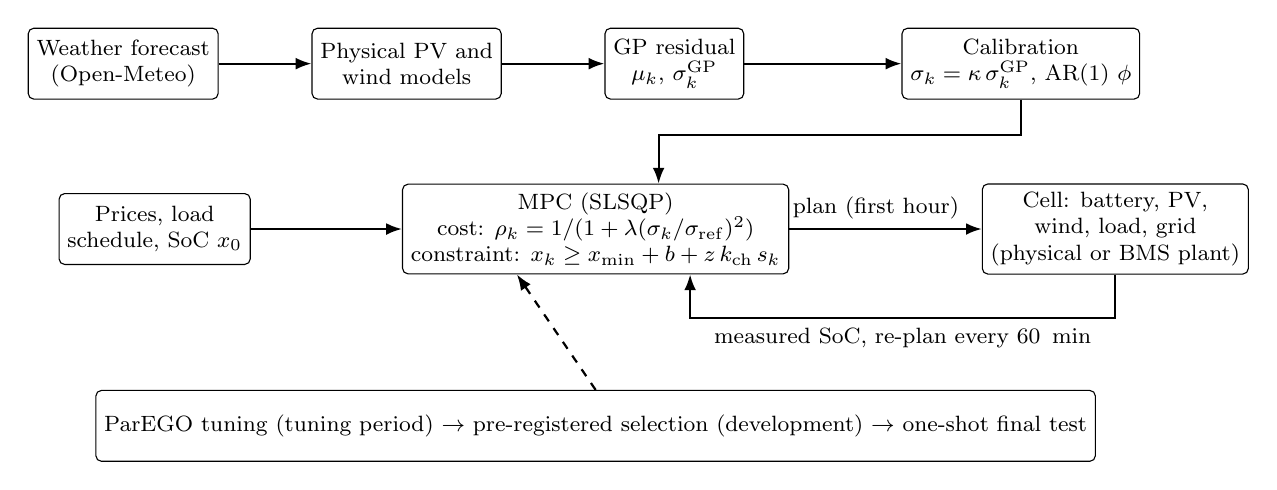
\begin{tikzpicture}[font=\footnotesize,
  box/.style={draw, rounded corners=2pt, align=center, minimum height=9mm, inner sep=3pt, fill=white},
  arr/.style={-{Latex[length=2mm]}, thick}]
\node[box] (wx) at (0,0) {Weather forecast\\(Open-Meteo)};
\node[box] (phys) at (3.6,0) {Physical PV and\\wind models};
\node[box] (gpr) at (7.0,0) {GP residual\\$\mu_k$, $\sigma^{\mathrm{GP}}_k$};
\node[box] (cal) at (11.4,0) {Calibration\\$\sigma_k=\kappa\,\sigma^{\mathrm{GP}}_k$, AR(1) $\phi$};
\node[box] (inputs) at (0.4,-2.1) {Prices, load\\schedule, SoC $x_0$};
\node[box, minimum width=48mm] (mpc) at (6.0,-2.1) {MPC (SLSQP)\\cost: $\rho_k=1/(1+\lambda(\sigma_k/\sigma_{\mathrm{ref}})^2)$\\constraint: $x_k\ge x_{\min}+b+z\,k_{\mathrm{ch}}\,s_k$};
\node[box] (plant) at (12.6,-2.1) {Cell: battery, PV,\\wind, load, grid\\(physical or BMS plant)};
\node[box] (tune) at (6.0,-4.6) {ParEGO tuning (tuning period) $\rightarrow$ pre-registered selection (development) $\rightarrow$ one-shot final test};
\draw[arr] (wx) -- (phys); \draw[arr] (phys) -- (gpr); \draw[arr] (gpr) -- (cal);
\draw[arr] (cal.south) -- ++(0,-0.45) -| ([xshift=8mm]mpc.north);
\draw[arr] (inputs) -- (mpc);
\draw[arr] (mpc.east) -- node[above, pos=0.45]{plan (first hour)} (plant.west);
\draw[arr] (plant.south) -- ++(0,-0.55) -| node[pos=0.25, below]{measured SoC, re-plan every \replanmin\,min} ([xshift=12mm]mpc.south);
\draw[arr, dashed] (tune.north) -- ([xshift=-10mm]mpc.south);
\end{tikzpicture}
\caption{Method. The calibrated forecast standard deviation enters the MPC twice: as the confidence weight $\rho_k$ in the cost and as the chance-constrained SoC margin. The controller weights are tuned in closed-loop replay and selected before the final test.}\label{fig:method}
\end{figure*}

\subsection{Renewable forecast}
For each channel (solar, wind) a GP learns the residual of the physical model, i.e.\ realised minus physical power, from forecast features: for solar the forecast irradiance, its change, its 3-h mean, the physical prediction and sine/cosine encodings of the hour and the day of year; for wind the forecast 10-m speed, its cube, change, 3-h mean and standard deviation, the 100-m speed, gusts, temperature, the physical prediction and the encoded hour and direction. The kernel is a scaled Matérn kernel ($\nu=1.5$) plus white noise \cite{rasmussen2006gaussian}, fitted with scikit-learn \cite{pedregosa2011scikit} on at most \gprsamples samples. The forecast mean is $\mu_k=\mu_{\mathrm{s},k}+\mu_{\mathrm{w},k}$ and its standard deviation $\sigma^{\mathrm{GP}}_k=(\sigma^2_{\mathrm{s},k}+\sigma^2_{\mathrm{w},k})^{1/2}$, assuming independent channels; the daytime correlation of the two errors on the calibration period was \swcorr.

\subsection{Calibration of the forecast uncertainty}
On the calibration period (\calhours forecast hours) the forecast RMSE was \calrmse\,W while the RMS of the GP standard deviation was \calrmssigma\,W: the raw GP was over-confident, covering \covRawOne\,\% and \covRawTwo\,\% of the errors with $\pm1\sigma$ and $\pm2\sigma$ (ideal 68.3 and 95.4\,\%). We therefore scale it, $\sigma_k=\kappa\,\sigma^{\mathrm{GP}}_k$, with $\kappa=\mathrm{RMSE}/\mathrm{RMS}(\sigma^{\mathrm{GP}})=\sigmascale$ \cite{gneiting2007probabilistic}. Forecast errors are correlated in time; the lag-1 autocorrelation of the standardised hourly errors was \phihour, i.e.\ $\phi=\phistep$ per \dtmin-min step, and we model the errors as an AR(1) process with $\mathrm{Cov}(e_i,e_j)=\sigma_i\sigma_j\phi^{|i-j|}$. A weather-dependent scale (a log-linear function of forecast gust excess and irradiance variability, fitted by maximum likelihood) was also tried; it is reported as a negative result in Section~\ref{sec:res:cal}.

\subsection{Uncertainty-aware MPC}\label{sec:mpc}
Every \replanmin\,min the controller solves, over $N=\horizon$ steps of $\Delta t=\dtmin$\,min, for the discharge $u^{\mathrm{dis}}_k$, the charge $u^{\mathrm{ch}}_k$ and the grid power $u^{\mathrm{g}}_k$. With $k_{\mathrm{ch}}=\eta\Delta t/E$ and $k_{\mathrm{dis}}=\Delta t/(\eta E)$ the SoC evolves as
\begin{equation}
x_{k}=x_0+\sum_{j\le k}\left(k_{\mathrm{ch}}u^{\mathrm{ch}}_j-k_{\mathrm{dis}}u^{\mathrm{dis}}_j\right).\label{eq:soc}
\end{equation}
The cost is
\begin{align}
J={}&w_x\sum_{k}(x_k-x_{\mathrm{ref}})^2\nonumber\\
&+\sum_k\left(p_k u^{\mathrm{g}}_k+c_{\mathrm{deg}}(u^{\mathrm{ch}}_k+u^{\mathrm{dis}}_k)\right)\Delta t\nonumber\\
&+w_{\Delta u}\sum_k\|\Delta u_k\|^2+w_{\mathrm{ff}}\sum_k\rho_k\left(u^{\mathrm{ch}}_k-\mu_k\right)^2\nonumber\\
&+w_T(x_N-x_{\mathrm{ref}})^2,\label{eq:cost}
\end{align}
with the day-ahead price $p_k$, $x_{\mathrm{ref}}=0.5$ and the increments $\Delta u_k$ of all three inputs. The fourth term is the uncertainty-aware weight of this paper:
\begin{equation}
\rho_k=\frac{1}{1+\lambda\left(\sigma_k/\sigma_{\mathrm{ref}}\right)^2},\label{eq:rho}
\end{equation}
which rewards charging that follows the forecast where the forecast is confident ($\rho_k\to1$) and releases the plan from it where the forecast is uncertain ($\rho_k\to0$), in the spirit of precision weighting. Dividing $\sigma_k$ by the installed renewable power $\sigma_{\mathrm{ref}}$ makes $\lambda$ dimensionless, so that the same $\lambda$ applies to systems of any size.

The constraints are the power balance $u^{\mathrm{g}}_k+u^{\mathrm{dis}}_k=D_k$, the limits $0\le u^{\mathrm{dis}}_k\le\min(\pdismax\,\mathrm{W},D_k)$, $0\le u^{\mathrm{ch}}_k\le\min(\pchmax\,\mathrm{W},\mu_k)$ and the tightened SoC band
\begin{align}
&x_{\min}+m_k\le x_k\le x_{\max},\nonumber\\
&m_k=\min\!\left(b+z\,k_{\mathrm{ch}}\,s_k,\ \tfrac{1}{2}(x_{\max}-x_{\min})-10^{-3}\right).\label{eq:margin}
\end{align}
Here $s_k$ is the standard deviation of the forecast errors accumulated over the $W$ steps up to step $k$,
\begin{equation}
s_k^2=\sum_{i=a_k}^{k}\sum_{j=a_k}^{k}\sigma_i\sigma_j\phi^{|i-j|},\quad a_k=\max(0,k-W+1),\label{eq:window}
\end{equation}
with $W$ equal to the re-planning interval (\replansteps steps). The errors accumulate only until the next re-planning, because each re-planning starts from the measured SoC. Accumulating them over the whole horizon, as in open-loop chance-constrained MPC, ignores this feedback and is conservative \cite{mesbah2016stochastic}. The upper limit is not tightened because charging is a decision variable and surplus renewable power is curtailed. The parameter $b$ is a constant back-off; with $z=0$ and $b>0$, \eqref{eq:margin} is the constant back-off baseline.

Three controllers share this formulation and differ only in what they use:
\DET (deterministic MPC: GP mean $\mu_k$, $\sigma_k=0$, $b=0$), \DETBO (as \DET with a tuned constant back-off $b$) and \UA (GP mean and calibrated $\sigma_k$, $b=0$, tuned $z$ and $\lambda$). Two ablations of \UA remove one use of $\sigma_k$ each: \emph{$\rho$ only} ($z=0$) and \emph{margin only} ($\lambda=0$, i.e.\ $\rho_k\equiv1$). An oracle MPC with the realised renewable power as forecast gives a lower bound on cost, and a grid-only and a rule-based controller (store all renewable energy, discharge to the load) are simple references.

\paragraph{SoC recovery} A disturbance can leave the measured SoC below $x_{\min}+m_0$. The band in \eqref{eq:margin} is then infeasible for the first steps and the solver fails. After the final test we added a recovery relaxation: the lower bound at step $k$ is lowered to the highest SoC reachable by step $k$ (full charging, no discharge beyond what the grid limit forces), and the relaxation can only shrink along the horizon. In normal operation it is zero. Unless stated otherwise, the results were computed without it; Section~\ref{sec:res:solver} reports its effect.

\paragraph{Solver} The problem is smooth with linear inequality constraints. It is solved with SLSQP \cite{kraft1988software} in SciPy \cite{virtanen2020scipy}, with analytic gradients and constraint Jacobians, normalised variables and an objective normalised to about one at the starting point. The solver is warm-started from the shifted previous plan; in the replay its tolerance is $\solverftol$.

\subsection{Closed-loop replay and violation metrics}\label{sec:replay}
Each controller runs in closed loop on the historical data: it plans from the forecast available at that time, the first \replanmin\,min of the plan are applied to the cell with the realised renewable power, and the next plan starts from the resulting SoC. The applied charge is limited by the realised renewable power and the applied discharge by the load. Two plants are simulated. The \emph{physical} plant only limits the SoC to $[0,1]$, so leaving the band $[x_{\min},x_{\max}]$ is measured as a violation. The \emph{BMS} plant adds a battery-management system that stops discharging at $x_{\min}$ and charging at $x_{\max}$; the grid covers the shortfall.

A constraint violation means three different things, and we report all three:
(1) leaving the planned band, measured on the physical plant as depth times duration,
\begin{equation}
V=100\sum_k\left(\max(x_{\min}-x_k,0)+\max(x_k-x_{\max},0)\right)\Delta t
\end{equation}
in percentage points times hours (pp$\cdot$h);
(2) the battery's own protection acting, counted as BMS protection steps; and (3) the consequence, the planned battery energy not delivered and its extra grid cost. The net cost is the grid and wear cost minus the value of the energy left in the battery at the end, valued at the mean price.

\subsection{Tuning with equal budget}\label{sec:tuning}
The weights $(w_x,w_{\mathrm{ff}},w_{\Delta u})$ and the controller-specific parameters ($b$ for \DETBO; $\lambda$, $z$ for \UA) are tuned by ParEGO \cite{knowles2006parego} on three objectives: net cost, SoC violation and curtailed renewable share; violations below \violNoise\pph count as zero. Each controller gets \trials evaluations: the configuration default, \initpoints Latin-hypercube points \cite{mckay1979comparison} and then expected-improvement proposals \cite{jones1998efficient} on an augmented Chebyshev scalarisation with random weights. One evaluation is a closed-loop replay of \episodes episodes of \episodeDays days (\episodeList) from the tuning period. Table~\ref{tab:space} lists the search space; $w_T=10^{-3}$ is fixed.

\begin{table}[t]
\caption{Search space of the tuning; sampled on a log scale except $^\dagger$ (linear).}\label{tab:space}
\small
\begin{tabular*}{\tblwidth}{@{}LLLL@{}}
\toprule
Param. & \DET & \DETBO & \UA \\
\midrule
\inputtab{tables/tab_space.tex}
\bottomrule
\end{tabular*}
\end{table}

\subsection{Evaluation protocol}\label{sec:protocol}
The tuning period yields a Pareto front per controller. Because a front point that is safe on 8 tuning days need not be safe elsewhere, every front point was replayed on the development period, and the operating point was chosen by a rule recorded on \prereqDate, before the final test was run: \emph{per controller, the cheapest development-period point whose violation is at most \thrPrimary\pph; if none qualifies, the point with the lowest violation}. A secondary threshold of \thrSecondary\pph was recorded as a sensitivity check. The final test was run once with the selected points, every variant on both plants, and each run was logged.

Differences are tested by a paired circular block bootstrap \cite{kunsch1989jackknife,politis1992circular,lahiri2003resampling} on the daily values of the two controllers (5-day blocks, 10\,000 resamples, full days only). We report the 95\,\% percentile interval of the total difference and the bootstrap share of resamples in which \UA is better.

\subsection{Decision indicators and map}\label{sec:map}
To describe when the forecast uncertainty matters, we use three indicators computed from the forecast and the realised power. With the forecast error $e_k=\mu_k-R_k$ (positive: less renewable power than forecast),
\begin{align}
\rE&=\frac{Q_{0.95}\left[\max\left(\sum_{j=k-W+1}^{k}e_j\Delta t,\,0\right)\right]}{E\,(x_{\max}-x_{\min})},\label{eq:rE}\\
\rP&=\frac{Q_{0.95}\left[\max(e_k,0)\right]}{\min(p^{\mathrm{dis}}_{\max},\max_kD_k)},\label{eq:rP}
\end{align}
and $\kappa_\sigma=\mathrm{std}(\sigma_k)/\mathrm{mean}(\sigma_k)$. $\rE$ is the energy deficit that can build up before the controller can react, relative to the usable capacity; it is directly comparable with the back-off $b$, which is also a fraction of the capacity. $\rP$ is the power dimension and $\kappa_\sigma$ the variability of the uncertainty over time.

The decision map replays \DETBO and \UA, both with their selected weights, on the development period while one condition changes at a time: capacity $E\in\{36,72,144\}$\,Wh, forecast-error level $s\in\{0.5,1,2\}$ (the error and the standard deviation are scaled, $\mu'_k=R_k+s(\mu_k-R_k)$, $\sigma'_k=s\sigma_k$) and, for the base cell, a re-planning interval of 4\,h instead of 1\,h. The map runs use the SoC recovery. Finally, \UA was replayed with $z\in\{0.5,1,1.645,2.326\}$ to compare the nominal per-step probability $\alpha=1-\Phi(z)$ with the observed share of steps below $x_{\min}$.

\paragraph{Variability experiment} Scaling the error leaves $\kappa_\sigma$ unchanged, so the map cannot separate the level of the uncertainty from its variation in time. In \varCells cells of the map (the base cell, 36\,Wh, doubled error level and 4-h re-planning) \UA was therefore replayed with the same weights and two modified standard deviations that keep the development-period mean $\bar\sigma$ of the total $\sigma_k$: a constant one, $\sigma'_k=\bar\sigma$ ($\kappa_\sigma=0$), and one with doubled deviations, $\sigma'_k=\max(\bar\sigma+2(\sigma_k-\bar\sigma),0)$ ($\kappa_\sigma=\kappaAmplified$; the clipping was never active). The split between the solar and wind channels is kept. The forecast mean and the realised power are unchanged, so any difference comes from where in time the margin is large.

\paragraph{Capacity economics} From the map cells with 1-h re-planning we compute, for each capacity and error level, the saving of \UA against grid-only operation over the development period (grid-only cost \gridOnlyDev\,\euro), the saving per watt-hour of capacity, its share of the saving of the 144-Wh battery and the marginal saving per added watt-hour.

%% =====================================================================================
\section{Results}\label{sec:results}

\subsection{Calibration}\label{sec:res:cal}
With the constant scale $\kappa=\sigmascale$, the calibrated forecast covered \covDevCAllOne\,\% and \covDevCAllTwo\,\% of the errors with $\pm1\sigma$ and $\pm2\sigma$ on the development period and \covFinCAllOne\,\% and \covFinCAllTwo\,\% on the final test (ideal 68.3 and 95.4\,\%); RMSE/$\sigma$ was \rtsDevCAll and \rtsFinCAll. On average the uncertainty is therefore slightly conservative. On the quarter of days with the largest forecast errors it is not: coverage dropped to \covDevCHardOne/\covDevCHardTwo\,\% (development) and \covFinCHardOne/\covFinCHardTwo\,\% (final test), with RMSE/$\sigma$ of \rtsDevCHard and \rtsFinCHard. The weather-dependent scale did not help: on the hard days of the final test it covered \covFinWHardOne/\covFinWHardTwo\,\%, worse than the constant scale. Part of the hard days look calm in the forecast itself, so a forecast-based scale cannot recognise them. We kept the constant scale.

\subsection{Tuning and point selection}\label{sec:res:tuning}
The tuning gave Pareto fronts of \frontDet (\DET), \frontDetbo (\DETBO) and \frontUa (\UA) points. Replayed on the development period (Fig.~\ref{fig:fronts}, Table~\ref{tab:fronts} in the appendix), the tuning-period violation was a poor predictor of the development-period violation (Spearman rank correlation \rankCorr over the \devPoints points): the \UA point t15, for instance, violated \uaFifteenTun\pph on the tuning episodes and \uaFifteenDev\pph on the development period. This is why the operating point was selected on the development period. No \DET point met the \thrPrimary\pph threshold. Of the \devFrontPoints points on the joint development-period front, \devFrontUa belong to \UA and one, the safest, to \DETBO. The pre-registered rule selected \DET~\selDet, \DETBO~\selBo and \UA~\selUa (Table~\ref{tab:weights}).

\begin{figure}[t]
\centering
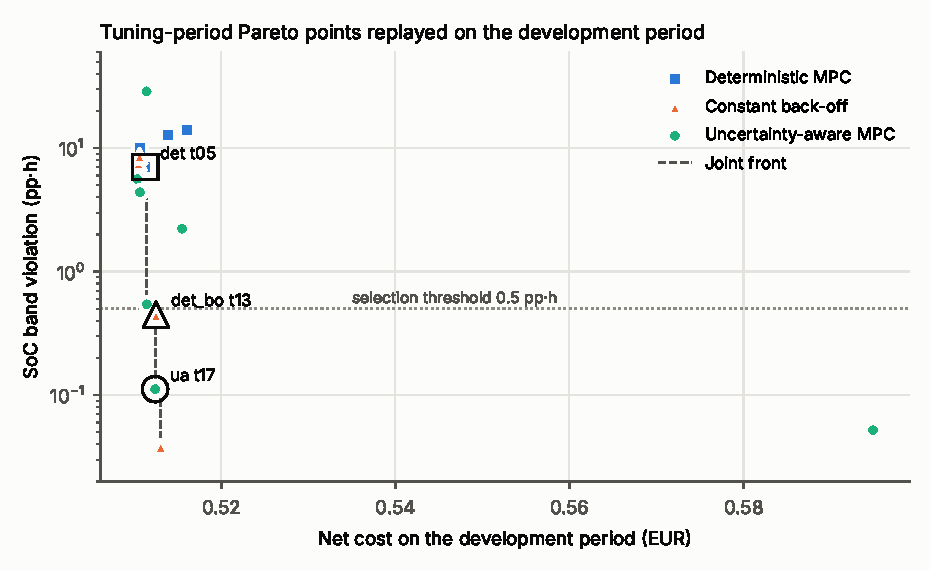
\includegraphics[width=\linewidth]{figures/fig1_dev_fronts.pdf}
\caption{Tuning-period Pareto points of the three controllers replayed on the development period (\daysDev days). Outlined: the points selected by the pre-registered rule; dashed: joint front; dotted: the \thrPrimary\pph threshold.}\label{fig:fronts}
\end{figure}

\begin{table*}[t]
\caption{Selected operating points (pre-registered rule) and their development-period result.}\label{tab:weights}
\begin{tabular*}{\tblwidth}{@{}LLLLLLRR@{}}
\toprule
Controller & Trial & $w_x$ & $w_{\mathrm{ff}}$ & $w_{\Delta u}$ & Specific & Net cost (\euro) & Violation (pp$\cdot$h) \\
\midrule
\inputtab{tables/tab_weights.tex}
\bottomrule
\end{tabular*}
\end{table*}

The tuned constant back-off of \DETBO is $b=\backoff$ (\backoffPct\,\% of the capacity). For \UA the tuner chose $z=\zUa$ (nominal $\alpha=\alphaUa$\,\%) and $\lambda=\lambdaUa$. On this system $\sigma_k/\sigma_{\mathrm{ref}}$ is small (median \sigRatioMed\,\%, 95th percentile \sigRatioNinetyFive\,\% on the development period), so this $\lambda$ gives $\rho_k\ge\rhoMinUa$: the confidence weight is practically inactive. The same holds for \frontLowLambda of the \frontUa \UA front points, whose $\lambda$ is below 10. We return to this in Section~\ref{sec:disc:rho}.

\subsection{Final test}\label{sec:res:final}
Table~\ref{tab:final} and Fig.~\ref{fig:final} give the \daysFin-day final test; Table~\ref{tab:boot} the paired bootstrap. The cell needed \finDemand\,kWh and received \finRenew\,kWh of renewable energy. \UA cost \finUaCost\,\euro, \finGridSaveUa\,\% less than supplying the load from the grid only and \finRuleSaveUa\,\% less than the rule-based controller; with a perfect (oracle) forecast the cost would have been \finOracleGap\,\% lower.

\begin{table*}[t]
\caption{Final test, \startFin to \stopFin (\daysFin days). Physical plant: net cost, SoC-band violation and its maximum depth; BMS plant: net cost, protection steps and the extra grid cost of the undelivered discharge; solver: share of converged solves (physical plant).}\label{tab:final}
\begin{tabular*}{\tblwidth}{@{}LRRRRRRR@{}}
\toprule
 & \multicolumn{3}{c}{Physical plant} & \multicolumn{3}{c}{BMS plant} & \\
\cmidrule(lr){2-4}\cmidrule(lr){5-7}
Controller & Net cost (\euro) & Violation (pp$\cdot$h) & Max depth (pp) & Net cost (\euro) & Protection steps & Extra grid cost (m\euro) & Solver (\%) \\
\midrule
\inputtab{tables/tab_final.tex}
\bottomrule
\end{tabular*}
\end{table*}

\begin{table*}[t]
\caption{Paired circular block bootstrap of the daily differences \UA minus the other controller over \finDaysBoot days (5-day blocks, 10\,000 resamples). Relative difference of the totals and 95\,\% interval of the total difference: cost in m\euro (grid and wear cost, physical plant), violation in pp$\cdot$h, protection in steps, extra grid cost in m\euro. $^{*}$: the interval excludes zero.}\label{tab:boot}
\begin{tabular*}{\tblwidth}{@{}LLLLL@{}}
\toprule
\UA vs. & Cost & Violation (physical) & Protection steps (BMS) & Extra grid cost (BMS) \\
\midrule
\inputtab{tables/tab_boot.tex}
\bottomrule
\end{tabular*}
\end{table*}

\begin{figure*}[t]
\centering
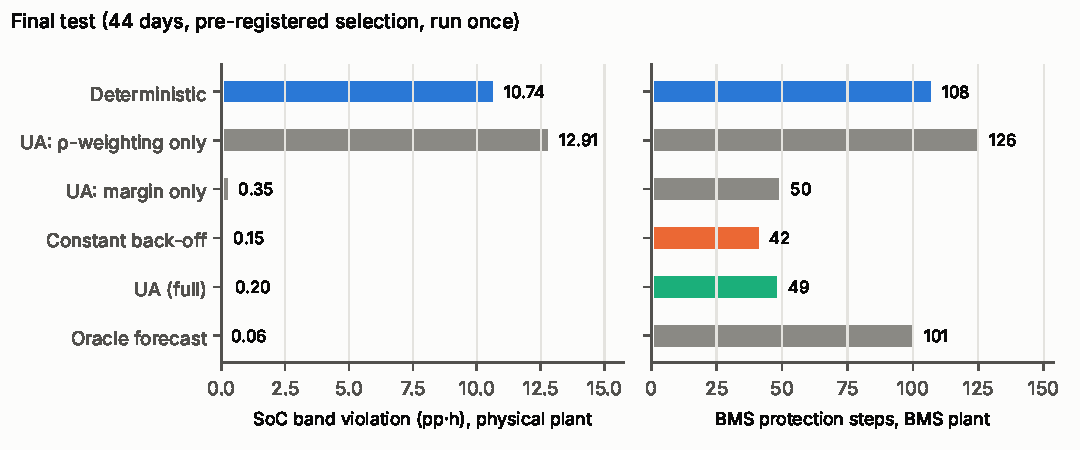
\includegraphics[width=0.85\textwidth]{figures/fig2_final_test.pdf}
\caption{Final test: SoC-band violation on the physical plant and battery-protection steps on the BMS plant.}\label{fig:final}
\end{figure*}

\paragraph{RQ1: against deterministic MPC} \UA reduced the SoC-band violation from \finDetViol to \finUaViol\pph (\btDetViolPct\,\%) and the BMS protection steps from \finDetProt to \finUaProt (\btDetProtPct\,\%); the extra grid cost of the undelivered discharge fell by \btDetExtraPct\,\%. All three intervals exclude zero. The cost difference was \btDetCostPct\,\% and not significant.

\paragraph{RQ2: against the tuned constant back-off} \DETBO violated \finBoViol\pph and \UA \finUaViol\pph; the bootstrap share in favour of \UA was \btBoViolP and the interval includes zero. On the BMS plant the protection steps were \finBoProt and \finUaProt (not significant). The extra grid cost was higher for \UA (\finUaExtra vs.\ \finBoExtra\,m\euro{} over \daysFin days), a significant but small difference. The costs were equal. In the setting it was tuned for, the constant back-off is as good as \UA.

\paragraph{Ablation} \UA with the $\rho$-weight only behaved like \DET (\finRhoViol\pph, \finRhoProt protection steps). \UA with the margin only reached \finMarginViol\pph and \finMarginProt steps, not significantly different from the full \UA. The safety effect comes from the margin; with the selected $\lambda$ the weight $\rho_k$ is close to one and adds no measurable effect (Section~\ref{sec:disc:rho}).

\paragraph{Sensitivity to the selection rule} With the secondary threshold (\thrSecondary\pph) the rule would have selected \UA~\selUaSec, which violated \finSecViol\pph on the final test. The choice of the operating point matters as much as the controller.

Fig.~\ref{fig:day} shows the hardest production day of the development period, \hardDay, with \hardErrWh\,Wh of absolute forecast error. In the morning the realised power stayed below the forecast while the load ran; \DET fell to \hardDetMinSoc\,\% SoC, \DETBO and \UA to \hardBoMinSoc and \hardUaMinSoc\,\%.

\begin{figure*}[t]
\centering
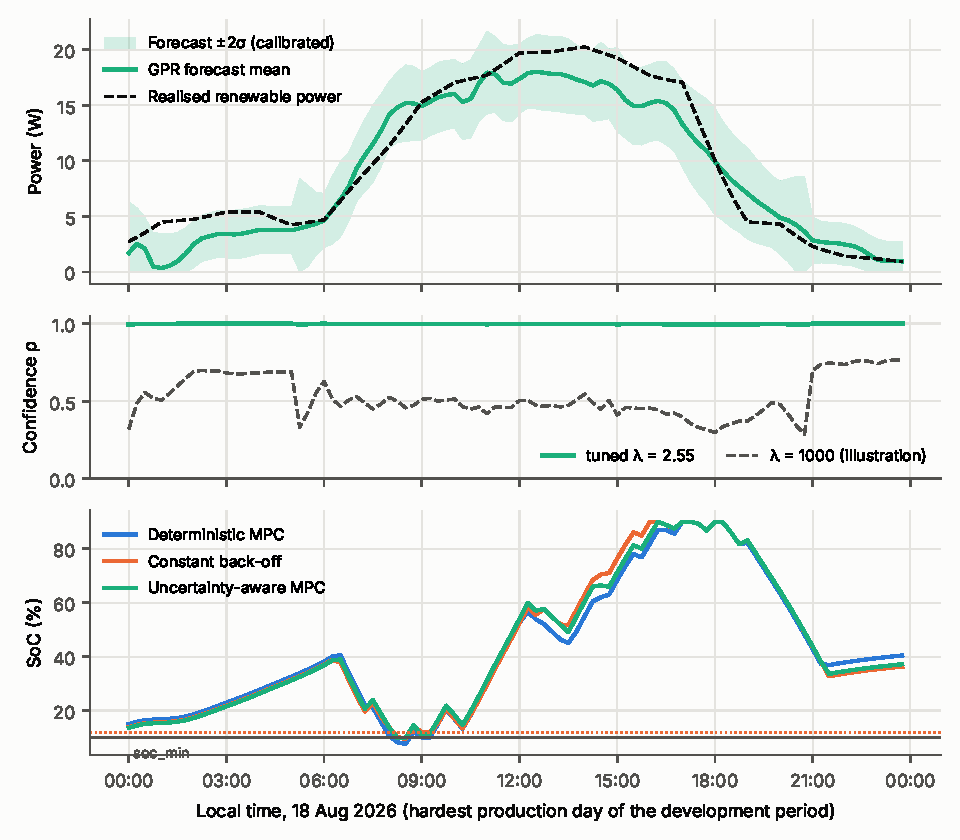
\includegraphics[width=0.78\textwidth]{figures/fig5_hard_day.pdf}
\caption{Hardest production day of the development period. Top: GP forecast with the calibrated $\pm2\sigma$ band and the realised renewable power. Middle: confidence weight $\rho_k$ for the tuned $\lambda$ and, for illustration, for $\lambda=1000$. Bottom: closed-loop SoC; solid line $x_{\min}$, dotted line $x_{\min}+b$ of \DETBO.}\label{fig:day}
\end{figure*}

\subsection{Decision map}\label{sec:res:map}
Fig.~\ref{fig:map} and Table~\ref{tab:map} show the map. In the base cell ($\Ecap$\,Wh, measured error level, 1-h re-planning) $\rE=\rEbase$, close to the tuned back-off $b=\backoff$. Wherever $\rE\le\mapLowThr$, both controllers kept the band (at most \mapLowMaxViol\pph) and the costs differed by at most \mapLowCostAbs\,\%. Wherever $\rE\ge\mapHighThr$, i.e.\ for the 36-Wh battery at the measured or doubled error level, the 72-Wh battery at the doubled error level and the 4-h re-planning, the constant back-off violated \mapHighBoMin--\mapHighBoMax\pph and \UA \mapHighUaMin--\mapHighUaMax\pph, \mapHighRatioMin--\mapHighRatioMax times less, at \mapHighCostMin--\mapHighCostMax\,\% extra cost. \UA used the same weights in every cell: its margin \eqref{eq:margin} grows with $\sigma_k$, with the window $W$ and with $1/E$ through $k_{\mathrm{ch}}$, while $b$ stays where it was tuned. The variability of the uncertainty, $\kappa_\sigma=\kappaSigma$, was the same in all cells, since scaling the error leaves it unchanged; Section~\ref{sec:res:var} tests it separately.

\begin{figure*}[t]
\centering
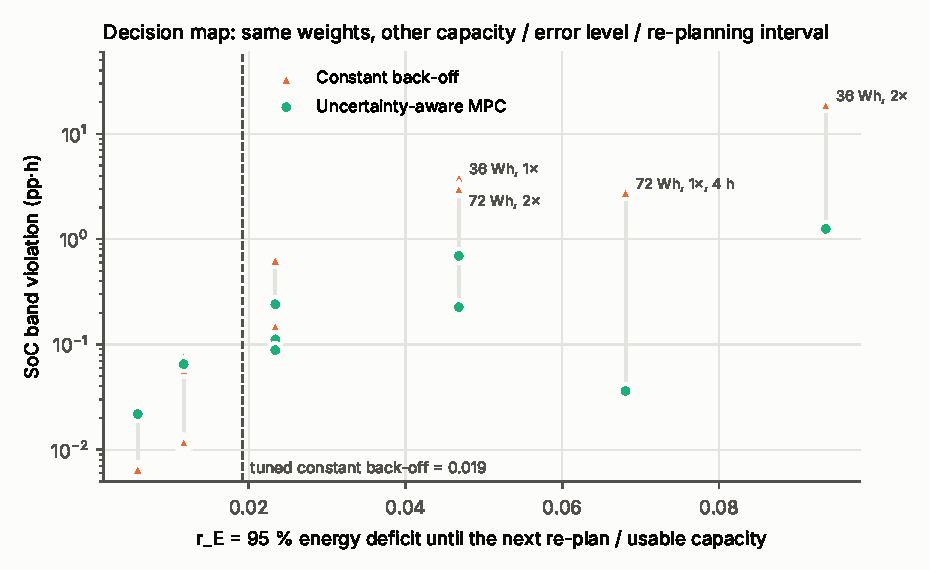
\includegraphics[width=0.72\textwidth]{figures/fig3_decision_map.pdf}
\caption{Decision map on the development period: SoC-band violation of the constant back-off and \UA against $\rE$, with the selected weights of both and the SoC recovery. Each vertical pair is one cell (capacity, error level, re-planning interval); the dashed line marks the tuned back-off.}\label{fig:map}
\end{figure*}

\begin{table*}[t]
\caption{Decision map: capacity $E$, error level $s$, re-planning interval, indicators $\rE$ and $\rP$, violation of \DETBO and \UA, and the cost difference of \UA relative to \DETBO.}\label{tab:map}
\begin{tabular*}{\tblwidth}{@{}RRRRRRRR@{}}
\toprule
$E$ (Wh) & $s$ & Re-plan (h) & $\rE$ & $\rP$ & \DETBO (pp$\cdot$h) & \UA (pp$\cdot$h) & $\Delta$cost (\%) \\
\midrule
\inputtab{tables/tab_map.tex}
\bottomrule
\end{tabular*}
\end{table*}

\subsection{Variability of the uncertainty}\label{sec:res:var}
Table~\ref{tab:var} and Fig.~\ref{fig:varcap}a compare \UA with its real standard deviation and with the two modified ones of equal mean. Holding $\sigma_k$ constant raised the violation \varConstRatioMin--\varConstRatioMax-fold in every cell; in the base cell from \varBaseUa to \varBaseConst\pph, above the tuned back-off. Doubling the variation lowered the violation \varAmpRatioMin--\varAmpRatioMax-fold in \varAmpLower of the \varCells cells (base cell: \varBaseAmp\pph) and raised it in the cell with 4-h re-planning (\varAmpWorseUa to \varAmpWorseAmp\pph). The costs of the three variants differed by at most \varCostSpreadMax\,\%. With the same average margin, it matters where in time the margin is placed. The result indicates that the real $\sigma_k$ is, on average, larger in the hours with larger forecast errors, so that a margin that follows it is large where it is needed; the one cell in which doubling the variation hurt shows that this alignment is imperfect. The constant-$\sigma$ variant still violated less than the constant back-off in \varConstBelowBo of the \varCells cells, because its margin \eqref{eq:margin} still grows with $1/E$, with the error level and with the window $W$. The adaptivity of \UA thus has two sources: the structure of the margin, which follows the operating conditions, and the time profile of $\sigma_k$, which follows the weather.

\begin{table*}[t]
\caption{Variability experiment on the development period: SoC-band violation (pp$\cdot$h) of the constant back-off and of \UA with constant $\sigma$ ($\kappa_\sigma=0$), the real $\sigma$ ($\kappa_\sigma=\kappaSigma$) and doubled variation ($\kappa_\sigma=\kappaAmplified$), all with the same mean $\sigma$ and the same weights; net cost of \UA with the real $\sigma$.}\label{tab:var}
\begin{tabular*}{\tblwidth}{@{}RRRRRRRRR@{}}
\toprule
$E$ (Wh) & $s$ & Re-plan (h) & $\rE$ & \DETBO & \UA, $\kappa_\sigma=0$ & \UA, real & \UA, doubled & Net cost (\euro) \\
\midrule
\inputtab{tables/tab_var.tex}
\bottomrule
\end{tabular*}
\end{table*}

\begin{figure*}[t]
\centering
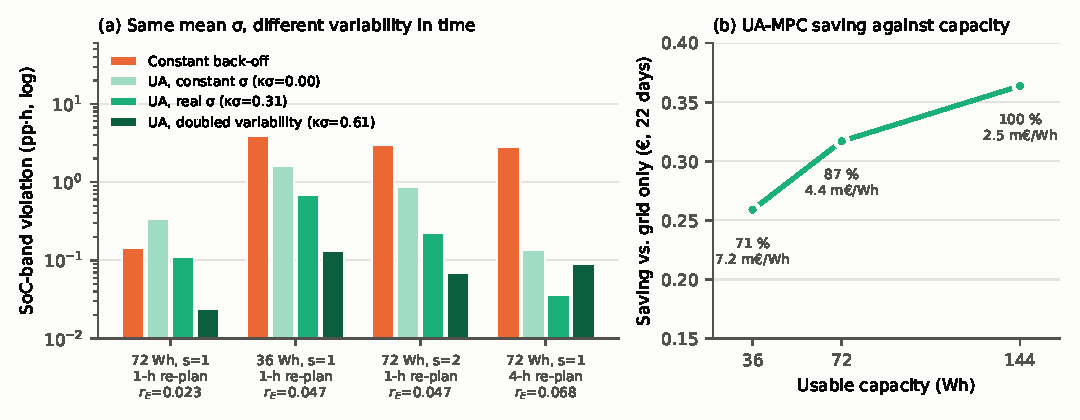
\includegraphics[width=0.9\textwidth]{figures/fig6_variability_capacity.pdf}
\caption{(a) SoC-band violation of the constant back-off and of \UA with the same mean forecast standard deviation but different variation in time (log scale). (b) Saving of \UA against grid-only operation over the \daysDev development days at the measured error level, with its share of the 144-Wh saving and the saving per watt-hour.}\label{fig:varcap}
\end{figure*}

\subsection{Capacity and the value of small batteries}\label{sec:res:cap}
Table~\ref{tab:cap} and Fig.~\ref{fig:varcap}b show the capacity economics. At the measured error level the 36-Wh battery saved \capSSave\,\euro against grid-only operation over \daysDev days, \capSShare\,\% of the \capLSave\,\euro saved by the 144-Wh battery with a quarter of its capacity (\capShareMin--\capShareMax\,\% over the three error levels). Per watt-hour the small battery earned \capSPerWh\,m\euro, the 72-Wh battery \capMPerWh and the 144-Wh battery \capLPerWh\,m\euro; the second 36\,Wh added \capMargMS\,m\euro/Wh and the last 72\,Wh \capMargLM\,m\euro/Wh. The small battery is also where the safety margin matters: it has the largest $\rE$, and the back-off tuned at 72\,Wh violated the band there by up to \mapHighBoMax\pph, \UA by at most \mapHighUaMax\pph without re-tuning.

\begin{table*}[t]
\caption{Capacity economics on the development period (1-h re-planning): saving of \UA against grid-only operation, its share of the 144-Wh saving, saving per watt-hour, marginal saving of the added capacity, and the violation of \DETBO and \UA.}\label{tab:cap}
\begin{tabular*}{\tblwidth}{@{}RRRRRRRRR@{}}
\toprule
$E$ (Wh) & $s$ & $\rE$ & Saving (\euro) & Share (\%) & m\euro/Wh & Marginal (m\euro/Wh) & \DETBO (pp$\cdot$h) & \UA (pp$\cdot$h) \\
\midrule
\inputtab{tables/tab_cap.tex}
\bottomrule
\end{tabular*}
\end{table*}

\subsection{Nominal and observed chance level}\label{sec:res:chance}
Increasing $z$ from 0.5 to 2.326 reduced the violation monotonically at a small cost increase (Table~\ref{tab:chance}, Fig.~\ref{fig:chance}). The observed share of steps below $x_{\min}$ was \chanceFacMin--\chanceFacMax times smaller than the nominal per-step $\alpha$. In closed loop, re-planning corrects most of the deviations before they reach the band edge, so $z$ is a tuning parameter, not a calibrated probability.

\begin{table*}[t]
\caption{\UA with different $z$ on the development period (\Ecap\,Wh, SoC recovery).}\label{tab:chance}
\begin{tabular*}{\tblwidth}{@{}RRRRR@{}}
\toprule
$z$ & Nominal $\alpha$ (\%) & Steps below $x_{\min}$ (\%) & Violation (pp$\cdot$h) & Net cost (\euro) \\
\midrule
\inputtab{tables/tab_chance.tex}
\bottomrule
\end{tabular*}
\end{table*}

\begin{figure}[t]
\centering
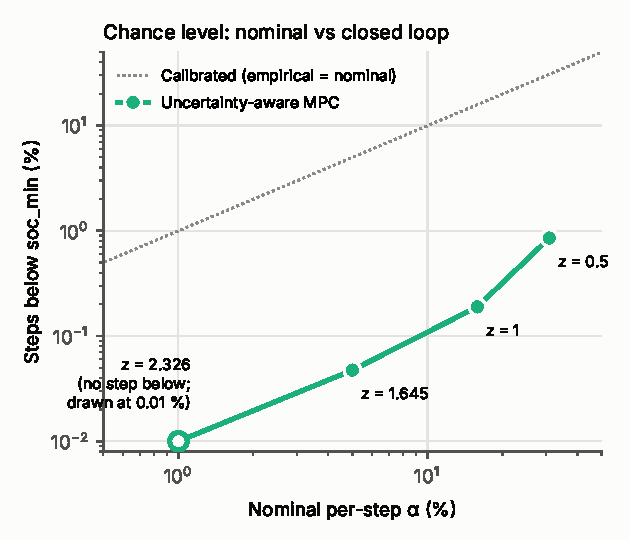
\includegraphics[width=0.8\linewidth]{figures/fig4_chance_calibration.pdf}
\caption{Nominal per-step $\alpha$ against the observed share of steps below $x_{\min}$ for \UA.}\label{fig:chance}
\end{figure}

\subsection{Solver behaviour and SoC recovery}\label{sec:res:solver}
In the development replays of the selected points, \solverFailMin--\solverFailMax\,\% of the solves did not converge. None of the \onsetsTotal violation onsets happened under a non-converged plan, but \violFailedMin--\violFailedMax\,\% of the violation accumulated under such plans: once the SoC is below the band, the start is infeasible and SLSQP iterates \iterFailedMin--\iterFailedMax times (median) instead of \iterOkMin--\iterOkMax without converging. Failures are a consequence of violations, which they prolong. With the SoC recovery the solvers converged in \recUaSolAfter--\recDetSolAfter\,\% of the solves; the violation changed from \recDetBefore to \recDetAfter\pph for \DET, from \recBoBefore to \recBoAfter\pph for \DETBO and not at all for \UA (\recUaBefore\pph); no cost changed by more than 0.01\,\%. The decision map (Section~\ref{sec:res:map}) uses the recovery; without it, two cells showed long shallow violations (\DETBO \oldOutBo\pph and \UA \oldOutUa\pph) that the recovery reduced to \newOutBo and \newOutUa\pph. The final test was run before the recovery was added and was not repeated.

The median solve time per plan was \finUaSolve\,s for \UA and \finDetSolve\,s for \DET on the final test, well within the \replanmin-min re-planning interval.

%% =====================================================================================
\section{Discussion}\label{sec:discussion}

\subsection{When is a constant back-off enough?}
The tuned back-off $b=\backoff$ and the base-cell $\rE=\rEbase$ are close: tuning found, implicitly, the energy deficit that builds up between two re-plannings in this cell. As long as the conditions stay where the back-off was tuned, a constant margin of that size does the job, and \UA brings no measurable advantage (RQ2). The value of \UA appears when the conditions move: a smaller battery, larger forecast errors or less frequent re-planning raise $\rE$ above $b$, and the constant margin becomes too small (RQ3). The uncertainty-aware margin follows these changes because each of them is a term of \eqref{eq:margin}--\eqref{eq:window}. A practical rule follows: compute $\rE$ from the forecast archive for the conditions the controller will meet; if $\rE$ can exceed the back-off one would tune, the uncertainty-aware margin removes the need to re-tune.

This is the same message as Kumar et al.\ \cite{kumar2019benchmarking}, that a constant back-off is ad hoc, made quantitative: the back-off is not wrong, it is specific to the conditions it was tuned for.

\subsection{Ratios as design rules and the case for small batteries}
Ratios such as self-sufficiency, capacity per annual load, the energy-to-power ratio or the battery size relative to a ramp limit \cite{luthander2015selfconsumption,weniger2014sizing,hesse2017lithium,makibar2017relation} are used to size storage before it is built. $\rE$ is their operational counterpart: the same capacity can be safe or unsafe for a given margin depending on the forecast quality and the re-planning interval, and $\rE$ puts the three into one number that can be compared directly with a back-off. Together with $\kappa_\sigma$ it describes the uncertainty a controller faces: $\rE$ its size relative to the battery, $\kappa_\sigma$ how unevenly it is spread in time. A constant back-off can match a large $\rE$ only by being large all the time; a margin that follows $\sigma_k$ can stay small where $\kappa_\sigma$ allows it (Section~\ref{sec:res:var}).

The capacity results connect this to the investment. Capacity has diminishing returns, as in the sizing literature \cite{weniger2014sizing,quoilin2016quantifying,mulleriyawage2020optimally}: here the first 36\,Wh earned more than ten times as much per watt-hour as the last 72\,Wh. An operator who wants the cheap, high-yield small battery accepts a large $\rE$, which is exactly the region where a constant back-off tuned for another battery fails and the self-adjusting margin keeps the band. Making small batteries safe to operate is therefore a way to make them usable, rather than buying capacity as a safety reserve.

\subsection{The confidence weight}\label{sec:disc:rho}
The confidence weight \eqref{eq:rho} is the element of the formulation without a direct precedent in MPC cost functions that we know of. On this cell the tuner made it inactive: with $\sigma_k/\sigma_{\mathrm{ref}}$ of a few percent, $\lambda\approx\lambdaUa$ gives $\rho_k\approx1$, and the ablations show no measurable effect of the weight. A larger $\lambda$ would vary $\rho_k$ strongly (down to \rhoMinDefault for $\lambda=1000$, Fig.~\ref{fig:day}) but was not preferred by the tuner. The reason is structural: in this formulation the weight only modulates how closely the planned charge follows the forecast, while the SoC risk is handled by the margin. We expect the weight to matter where following the forecast itself is costly, e.g.\ with expensive curtailment or a binding grid-export limit, or where $\sigma_k$ is a large share of the installed power. The scale-free form makes such a transfer straightforward, but this paper does not demonstrate a benefit of the weight.

\subsection{Evaluation practice}
Two observations concern the method of evaluation more than the controllers. First, a Pareto point that is safe on the tuning episodes is not necessarily safe elsewhere (rank correlation \rankCorr); a point-selection rule on separate data, fixed before the test, is necessary. Second, the solver failures were a symptom of violations, not their cause; reporting convergence together with the violation onsets avoids misattributing them. The three-level metric makes the cost of a violation visible: on the BMS plant the band is never left, but the protection steps and the extra grid cost show the same ranking as the violation on the physical plant.

\subsection{Limitations}
The final test covers \daysFin autumn days at one site; seasons with more wind or longer periods of poor forecasts were not tested, and slow changes (battery ageing, drift of the forecast model) were not studied. The calibration is weakest on the hardest days, which is where the margin matters most. The decision map covers capacity, error level and re-planning interval but not the temporal correlation of the errors, and its error scaling keeps the shape of the real errors; the variability experiment changes the time profile of $\sigma_k$ but not that of the errors themselves, and covers \varCells cells. The capacity economics use one load profile, one price period and the wear cost of this study, without investment costs; they show the shape of the returns, not a sizing recommendation. The wear model is linear in throughput, a first-order approximation of cycle-depth-dependent ageing \cite{xu2018factoring}. The load is assumed known. The cell is laboratory-scale; the dimensionless quantities ($\sigma_k/\sigma_{\mathrm{ref}}$, $\rE$, $b$) transfer to larger systems, but an industrial-scale case and measurements on the physical line are still needed. Numerical details matter at the level of single violations: re-running one development cell with single-threaded instead of multi-threaded linear algebra changed the \DETBO violation from \devAblBoViol to \mapBaseBoSingle\pph, while \UA was unchanged. The final-test runs were interrupted once by a time limit and resumed single-threaded; the physical-plant runs of \DET, \DETBO and \UA with $\rho$ only had finished before, all other runs were made after. Such shifts do not affect the comparison with \DET, which differs by two orders of magnitude, but they are of the size of the difference between \UA and \DETBO, which was not significant. Scenario-based and robust (tube) MPC were not compared.

%% =====================================================================================
\section{Conclusions}\label{sec:conclusion}
An uncertainty-aware MPC that uses a calibrated forecast standard deviation as a chance-constrained SoC margin, accumulated only until the next re-planning, kept the SoC band of a renewable-powered production cell far better than deterministic MPC at the same cost: \btDetViolPct\,\% less violation and \btDetProtPct\,\% fewer battery-protection interventions in a pre-registered, one-shot final test. Against a constant back-off tuned for the same setting with the same budget it was not better. Its advantage is that it adjusts itself: when the battery capacity, the forecast-error level or the re-planning interval changed, the same weights kept the band while the constant back-off violated it by up to \mapHighBoMax\pph. The ratio $\rE$ of the 95\,\% energy deficit until the next re-plan to the usable capacity tells an operator in advance whether a constant back-off will be enough. The time variability of the forecast uncertainty matters on its own: with the same mean, a constant standard deviation gave \varConstRatioMin--\varConstRatioMax times more violation. Because small batteries earn the most per watt-hour but have the largest $\rE$, the self-adjusting margin is most useful exactly where capacity is scarce. The confidence weight in the cost is available in the formulation but was not used by the tuner on this system. Future work will test the controller over several seasons, on the physical production line and at industrial scale, and against scenario-based and robust MPC.

%% =====================================================================================
\section*{Data and code availability}
The controller, the replay, the tuning and all evaluation scripts are in the project repository (TODO: link or DOI). The numbers and tables of this paper are generated from the result files by \url{paper/manuscript/scripts/make_numbers.py}; the result files, the pre-registration record and the log of final-test runs are part of the results package (TODO: archive DOI).

\section*{Declaration of competing interest}
The authors declare that they have no known competing financial interests or personal relationships that could have appeared to influence the work reported in this paper.

\section*{Declaration of generative AI and AI-assisted technologies in the manuscript preparation process}
% TODO: check and adapt to the journal's current wording
During the preparation of this work the authors used Claude (Anthropic) to assist with code development, the evaluation scripts and drafting of the text. After using this tool, the authors reviewed and edited the content as needed and take full responsibility for the content of the published article.

\printcredits

\appendix
\section{Development-period fronts}\label{app:fronts}

\begin{table}[h]
\caption{Pareto points of the tuning period replayed on the development period. $\star$: selected by the pre-registered rule; joint: on the joint development-period front.}\label{tab:fronts}
\begin{tabular*}{\tblwidth}{@{}LLRRRRL@{}}
\toprule
 & & \multicolumn{2}{c}{Tuning} & \multicolumn{2}{c}{Development} & \\
Controller & Trial & Cost (\euro) & Viol. & Cost (\euro) & Viol. & Joint \\
\midrule
\inputtab{tables/tab_fronts.tex}
\bottomrule
\end{tabular*}
\end{table}

\section{Development-period ablation with the tuning-period points}\label{app:devabl}
Before the selection rule was defined, the ablation was run on the development period with the tuning-period \emph{balanced} points (Table~\ref{tab:devabl}). It showed the same ranking of the variants as the final test and that the tuning-period points generalised poorly, which led to the selection rule of Section~\ref{sec:protocol}.

\begin{table}[h]
\caption{Development period, tuning-period balanced points (\DET t15, \DETBO t13, \UA t01).}\label{tab:devabl}
\begin{tabular*}{\tblwidth}{@{}LRRRR@{}}
\toprule
 & \multicolumn{2}{c}{Physical} & \multicolumn{2}{c}{BMS} \\
Controller & Cost (\euro) & Viol. (pp$\cdot$h) & Cost (\euro) & Prot. steps \\
\midrule
\inputtab{tables/tab_devabl.tex}
\bottomrule
\end{tabular*}
\end{table}

\section{Reproduction}\label{app:repro}
All commands are run from the repository root. Tuning, for each controller \texttt{det}, \texttt{det\_bo} and \texttt{ua}:
\begin{verbatim}
python src/tune_mpc.py --controller ua
  --trials 30 --episodes 4 --episode-days 2
  --set SoC.E_capacity=72
  --set degradation.c_deg=2e-5
\end{verbatim}
The development fronts, the ablation, the solver check, the pre-registration, the final test and the decision map are produced by the scripts in \url{results/paper/scripts}. The numbers, tables and figures of this paper are then produced by \url{paper/manuscript/scripts/make_numbers.py}, \url{figures.py} and \url{fig_day.py}.

\bibliographystyle{unsrtnat}
\bibliography{refs}

\end{document}
